%!TEX root = ./jctt.tex

\section{Computational Results}
\begin{figure}
\centering
\begin{subfigure}{.515\textwidth}
	\centering
	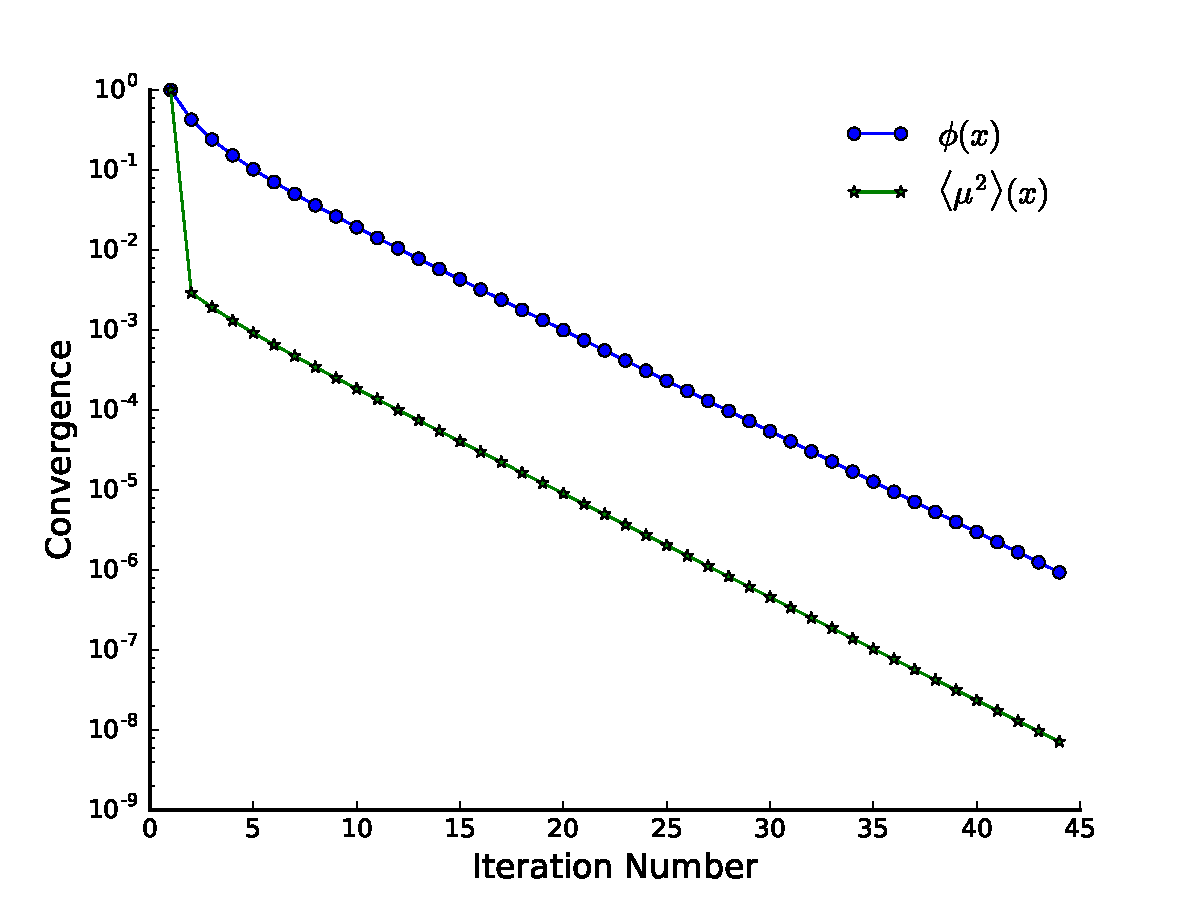
\includegraphics[width=\textwidth]{figs/si.pdf}
	\caption{}
	\label{fig:si}
\end{subfigure}
\hspace{-2em}
\begin{subfigure}{.515\textwidth}
	\centering
	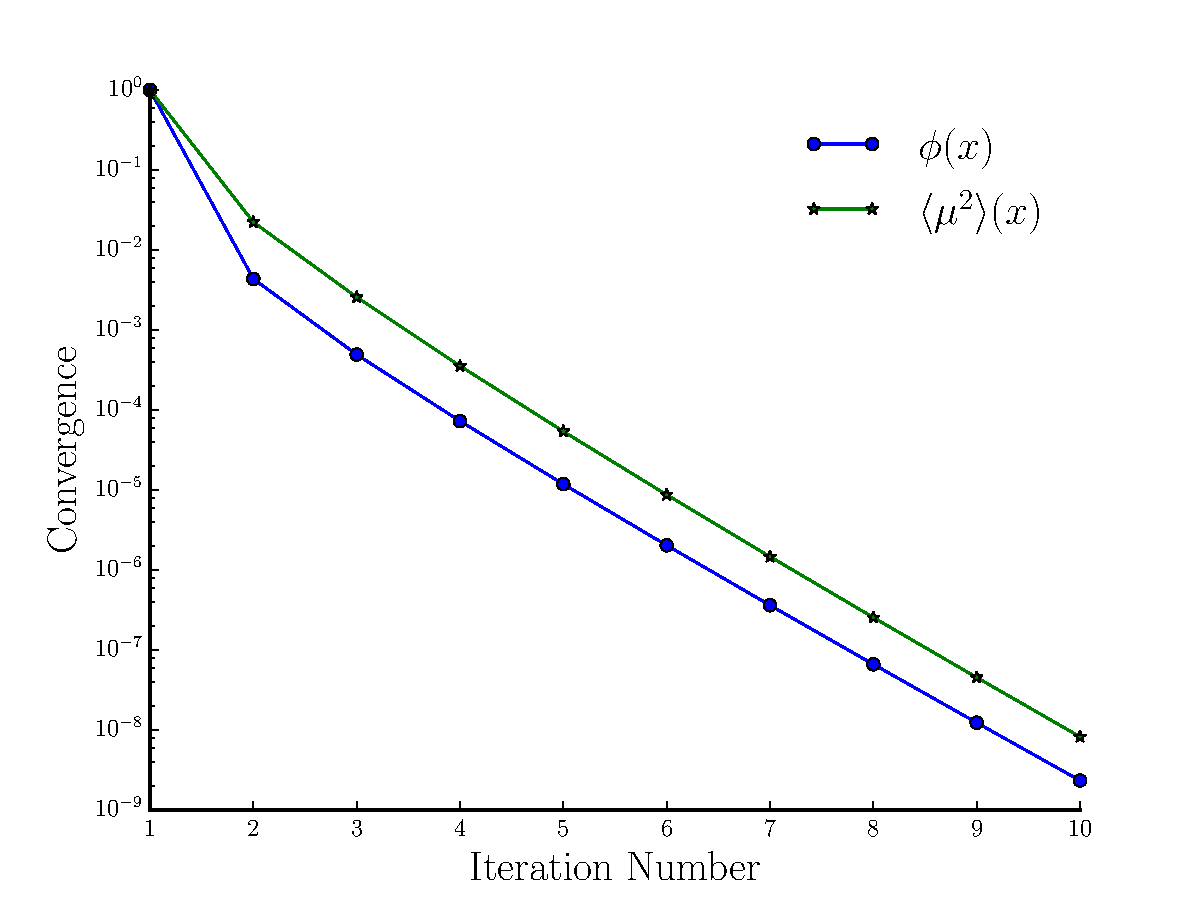
\includegraphics[width=\textwidth]{figs/vef.pdf} 
	\caption{}
	\label{fig:vef}
\end{subfigure}
\caption{The convergence rate for $\phi(x)$ and $\edd(x)$ for (a) unaccelerated and (b) VEF accelerated SI. }
\end{figure}

Figure \ref{fig:si} shows the convergence criterion
	\begin{equation}
		\frac{\| f\relll - f^\ell \|}{\| f\relll \|} 
	\end{equation}
as a function of unaccelerated iteration number for $f = \phi(x)$ and $f = \edd(x)$. The large drop in the convergence criterion between the first and second iterations supports the claim that the angular shape of the angular flux, and thus the Eddington factor, converges rapidly. When compared to Fig. \ref{fig:vef}, a plot of the convergence criterion versus number of iterations for the VEF method, it is clear that the VEF method transfers the fast rate of convergence of the Eddington factor to the scalar flux. 

	% \begin{figure}
	% 	\centering
	% 	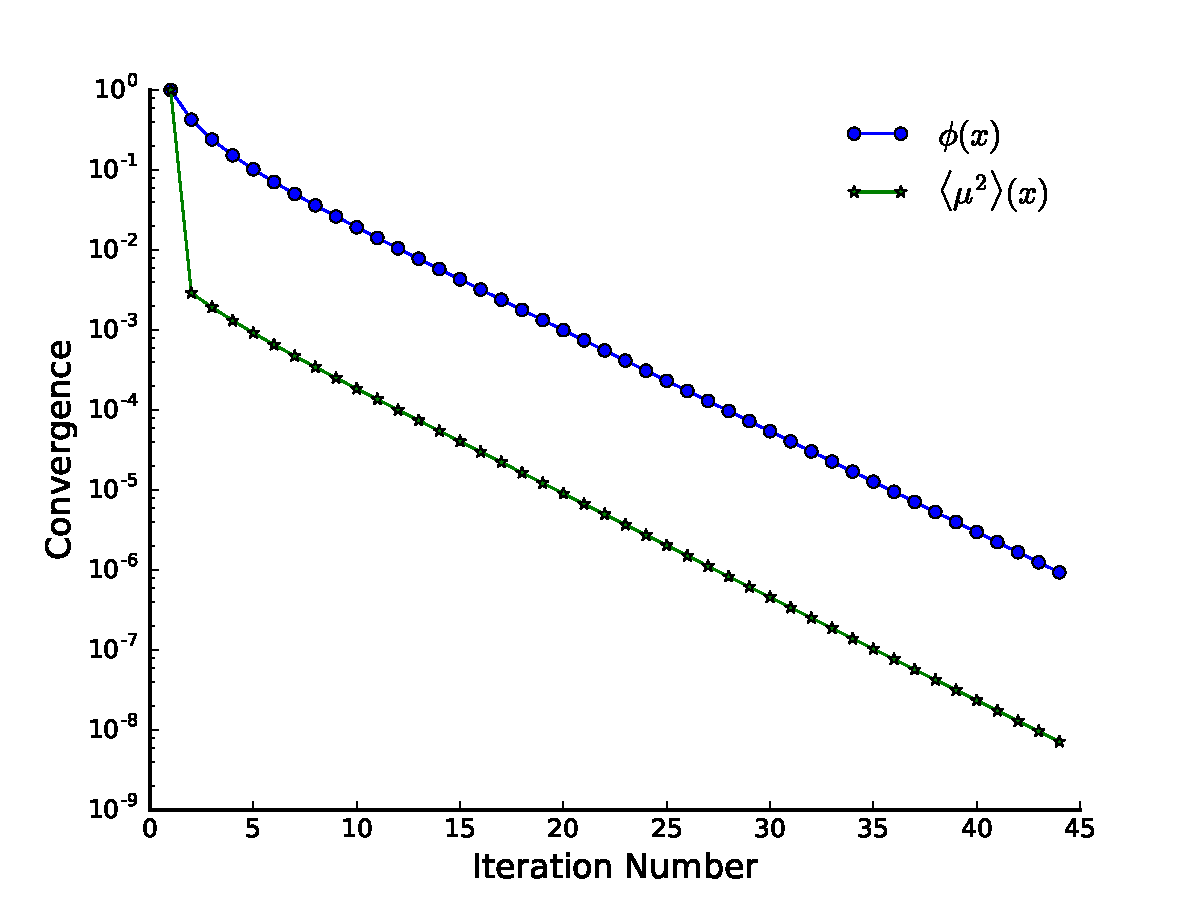
\includegraphics[width=.75\textwidth]{figs/si.pdf}
	% 	\caption{The convergence rate for $\phi(x)$ and $\edd(x)$ for unaccelerated S$_8$ Source Iteration. }
	% 	\label{fig:si}
	% \end{figure}

	% \begin{figure}
	% 	\centering
	% 	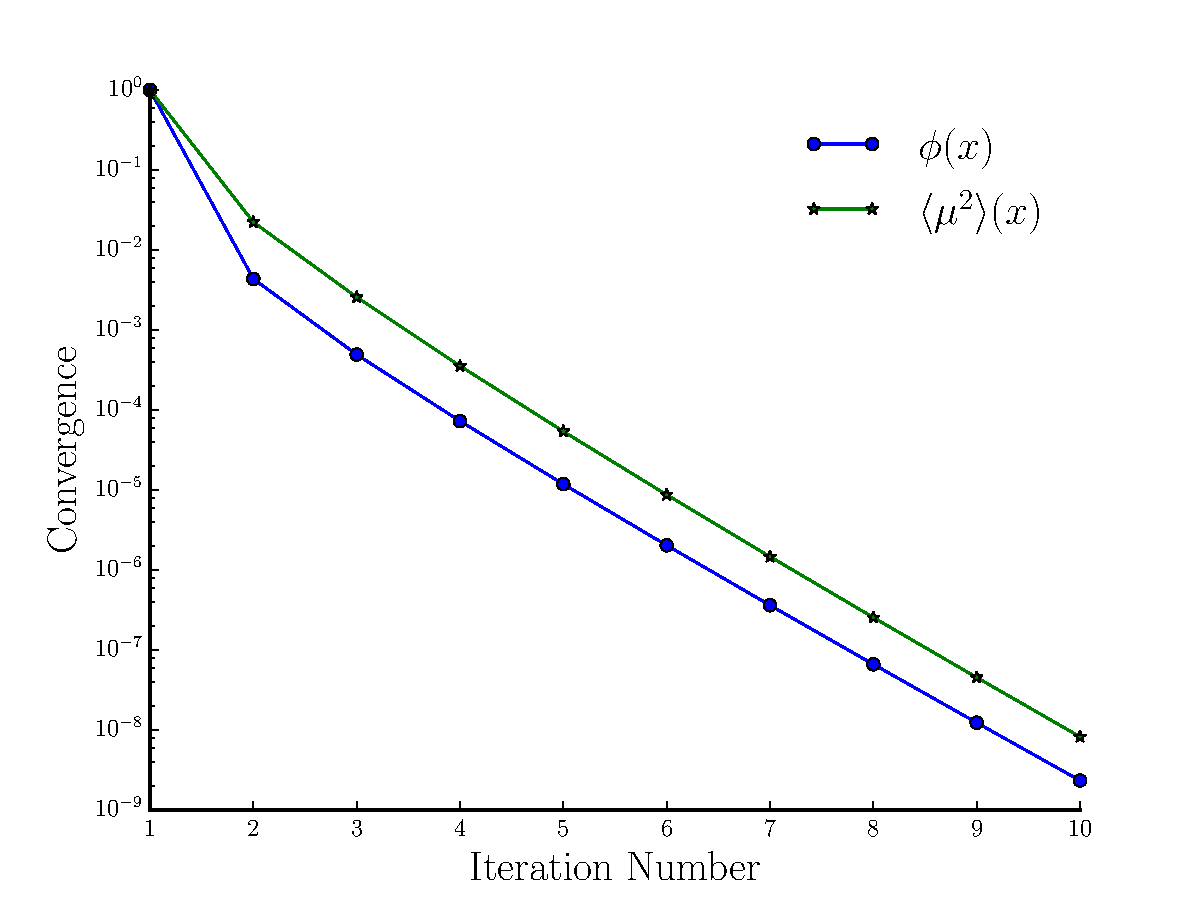
\includegraphics[width=.75\textwidth]{figs/vef.pdf} 
	% 	\caption{The convergence rate for $\phi(x)$ and $\edd(x)$ for VEF accelerated S$_8$. }
	% 	\label{fig:vef}
	% \end{figure}

To compare SI, VEF, and consistently differenced S$_2$SA, a test problem with a reflecting left boundary and a vacuum right boundary was used. This system was discretized into 50 spatial cells. $\sigma_t$ was set to \SI{1}{cm^{-1}} leading to an optical thickness per cell of 0.2. The convergence tolerance was set to \num{e-6}. Figure \ref{fig:si_vef_s2sa} shows the number of iterations required for convergence for SI, VEF, and S$_2$SA for varying ratios of $\sigma_s$ to $\sigma_t$. Aside from $\sigma_s/\sigma_t = 0$ where acceleration is not possible, the ratio of unaccelerated to VEF accelerated iterations ranged from 1.6 to 7. This suggests that acceleration is occurring and that the VEF method is not just doing twice the amount of work per iteration. In addition, the VEF method performed similarly to S$_2$SA. 

	\begin{figure}
		\centering
		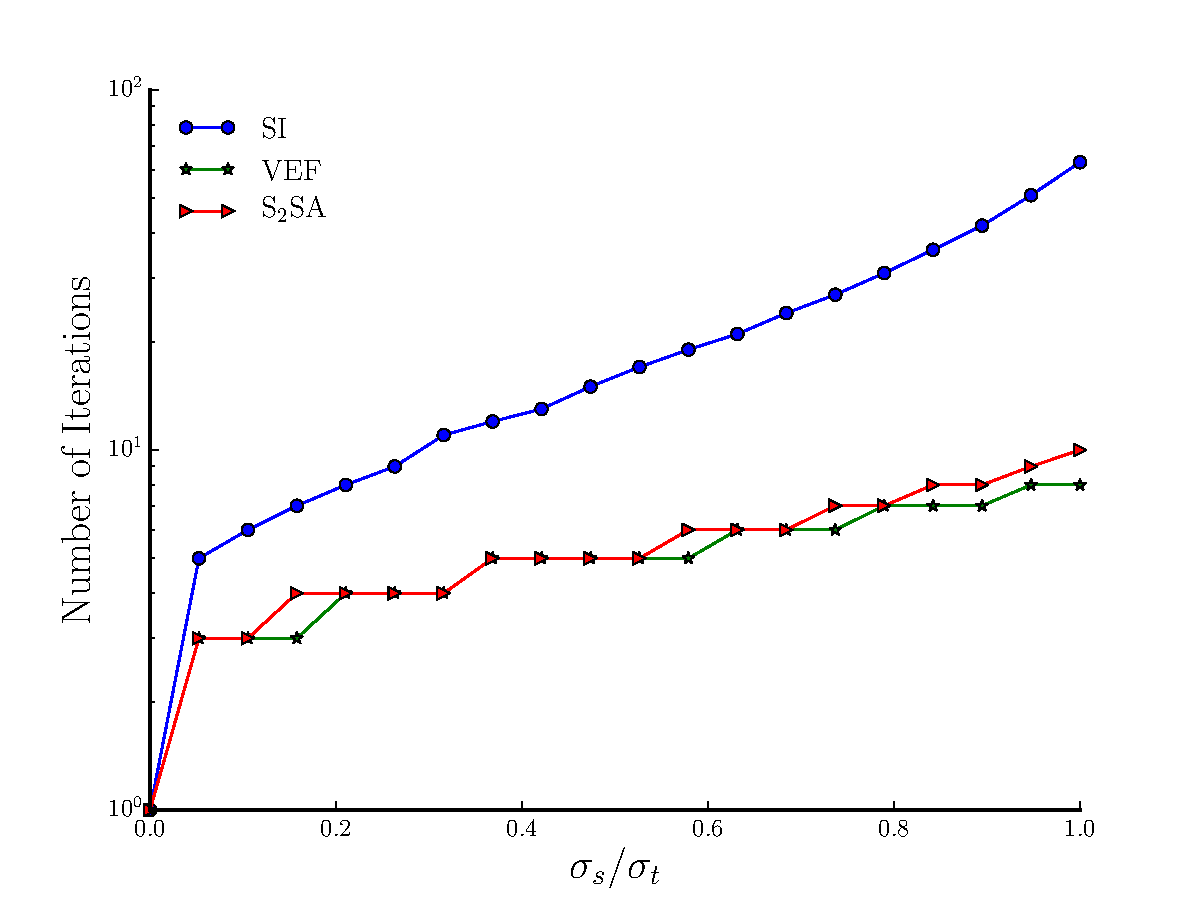
\includegraphics[width=.75\textwidth]{figs/si_vef_s2sa.pdf} 
		\caption{A comparison of the number of iterations required for Source Iteration, VEF acceleration, and S$_2$SA to converge for varying ratios of $\sigma_s$ to $\sigma_t$. } 
		\label{fig:si_vef_s2sa}
	\end{figure}

The Method of Manufactured Solutions (MMS) was used to compare the accuracy of the VEF method as the cell width was decreased. The L2 norm of the difference between the numerical and MMS solutions was compared at five logarithmically spaced cell widths between \SI{0.5}{mm} and \SI{0.01}{mm}. A line of best fit of the form 
	\begin{equation}
		E = C h^n
	\end{equation}
was used to find the order of accuracy, $n$, and the constant of proportionality, $C$, of the numerical error, $E$. These values are provided in Table \ref{tab:mms} for the permutations of the two reconstruction methods and two angular flux representation methods. All of the permutations are second order accurate and have similar overall accuracy. This suggests that slope reconstruction and angular flux representation do not affect numerical accuracy. It is also a testament to the robustness of the VEF method as the inconsistent, partially consistent, and fully consistent methods all performed similarly. 

	\begin{table} \centering
	\begin{tabular}{|c|c|c|c|c|}
	\hline
	\hline
	Reconstruction Method & $\psi$ Representation & Order & $C$ & $R^2$ \\ 
	\hline
		Flat & \num{1.979} & \num{1.18} & \num{9.9999e-01} \\
Linear & \num{1.988} & \num{0.786} & \num{9.9887e-01} \\

	\hline
	\hline
	\end{tabular}
	\caption{The order of accuracy, error, and $R^2$ values for the permutations of the two Eddington representation methods and two slope reconstruction methods. }
	\label{tab:mms}
	\end{table}
	\afterpage{\clearpage}

The convergence between unaccelerated SI and the VEF method was compared as a function of cell width for a simple homogeneous slab and for Reed's problem. In both cases, the left boundary was reflecting and the right boundary was vacuum. The homogeneous slab had a scattering ratio of 0.75. The cross sections and source for Reed's problem are provided in Table \ref{tab:reedXS}. The L2 norm of the difference between the SI solution and VEF solution is plotted for the four permutations of no reconstruction, van Leer slope limited reconstruction, constant angular flux representation, and linear angular flux representation in Figures \ref{fig:homo} and \ref{fig:reed} for the homogeneous slab problem and Reed's problem. 

	\begin{table} \centering
		\begin{tabular}{|c|c|c|c|c|c|}
			\hline
			& Region 1 & Region 2 & Region 3 & Region 4 & Region 5 \\ 
			\hline 
			$q$ & 50 & 0 & 0 & 0 & 1 \\ 
			$\Sigma_t$ & 50 & 0.001 & 1 & 5 & 1 \\ 
			$\Sigma_a$ & 50 & 0 & 0.1 & 0 & 0.1 \\ 
			\hline 
			Domain & $0 \leq x < 2$ & $2 \leq x < 4$ & $4\leq x < 6$ &
				$6 \leq x < 7$ & $7 \leq x \leq 8$\\ 
			\hline 
		\end{tabular}
		\caption{The cross sections and source used for Reed's problem.}
		\label{tab:reedXS}
	\end{table}

	\begin{figure}
		\centering
		\begin{subfigure}{.5\textwidth}
			\centering
			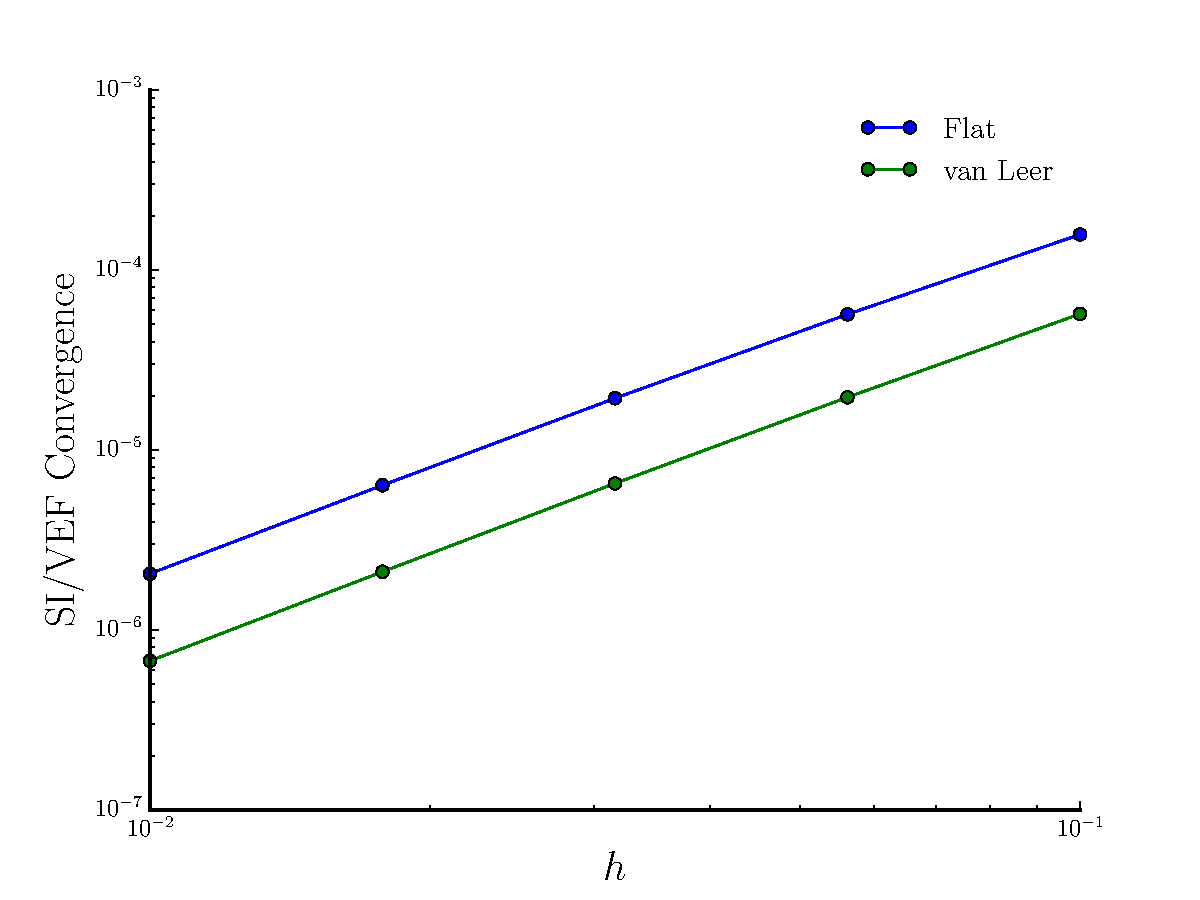
\includegraphics[width=\textwidth]{figs/solconv_homo.pdf}
			\caption{}
			\label{fig:homo}
		\end{subfigure}
		\hspace{-2em}
		\begin{subfigure}{.5\textwidth}
			\centering
			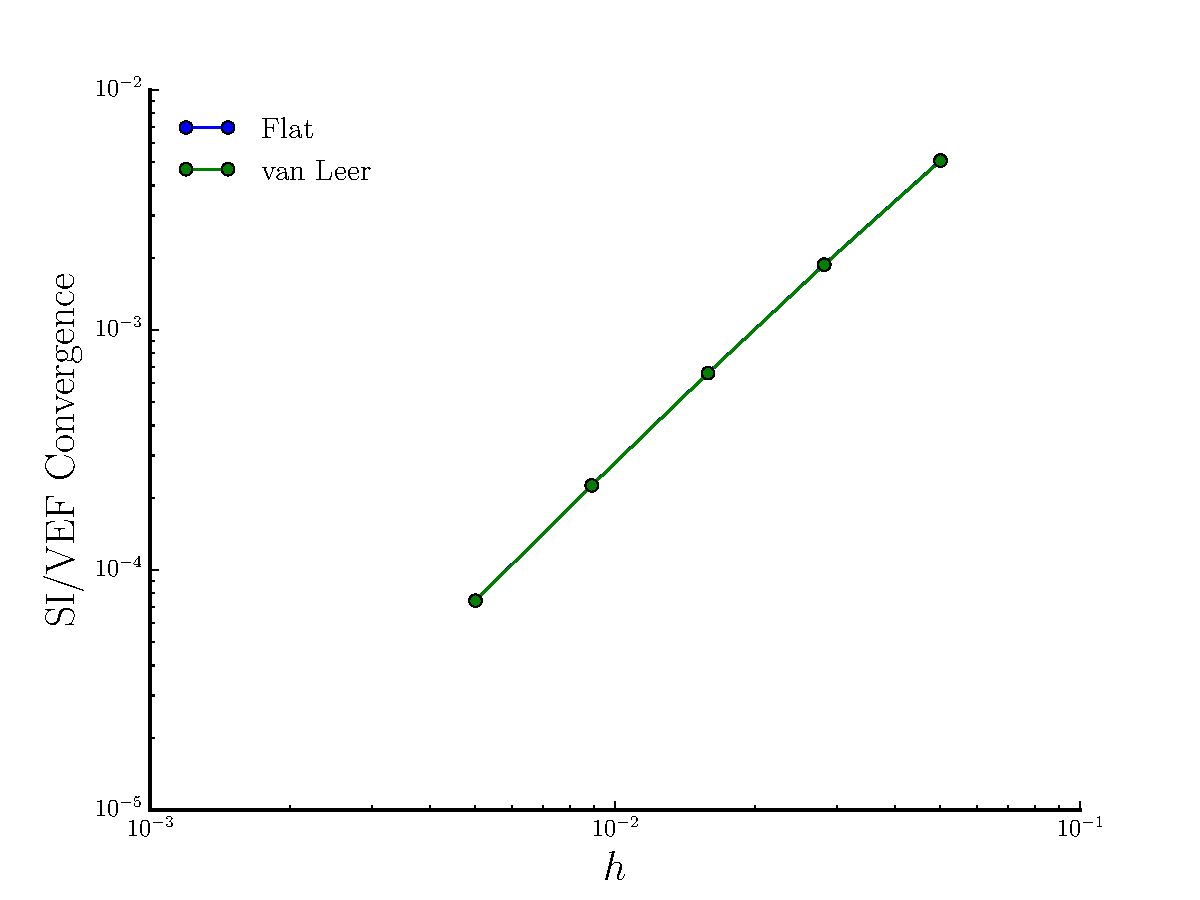
\includegraphics[width=\textwidth]{figs/solconv_reed.pdf}
			\caption{}
			\label{fig:reed}
		\end{subfigure}
		\caption{The L2 norm of the difference between SI and the four permutations of the VEF method as the cell spacing is decreased for (a) the homogeneous slab problem and (b) Reed's problem. }
	\end{figure}

In the homogeneous problem, VEF with van Leer limited slope reconstruction was five times more convergent than VEF without reconstruction. Use of the linear angular flux representation decreased the van Leer reconstruction convergence by 30\%. In Reed's problem, all four methods performed similarly. This suggests that the effects ofa angular flux respresentation and slope reconstruction are problem dependent. 

Lastly, slope reconstruction and angular flux representation were tested in the diffusion limit. The cross sections and source were scaled according to: 
	\begin{subequations} \label{res:scaling}
		\begin{equation} 
			\sigma_t(x) \rightarrow \sigma_t(x)/\epsilon \,, 
		\end{equation}
		\begin{equation}
			\sigma_s(x) \rightarrow \epsilon \sigma_s(x) \,,
		\end{equation}
		\begin{equation}
			Q(x) \rightarrow \epsilon Q(x) \,. 
		\end{equation}
	\end{subequations}
As $\epsilon \rightarrow 0$, the system becomes diffusive. The number of iterations for convergence within a tolerance of \num{e-10} as $\epsilon \rightarrow 0$ is plotted in Fig. \ref{fig:dl_it}. The error between the VEF solution and the exact diffusion solution is provided in Fig. \ref{fig:dl_err}. This supports the claim that the VEF method is robust as all four permutations survived the diffusion limit. 
	
	\begin{figure}
		\centering
		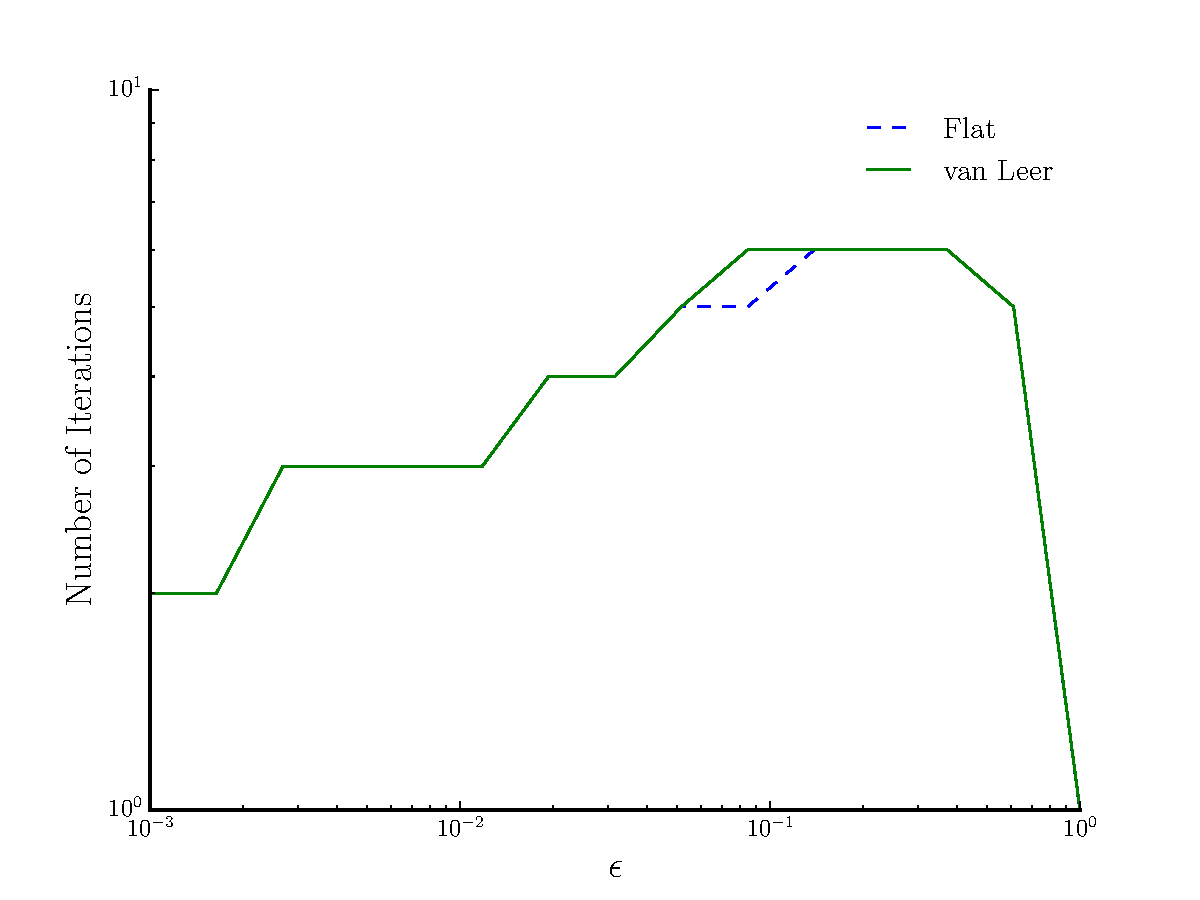
\includegraphics[width=.75\textwidth]{figs/dl_it.pdf}
		\caption{The number of iterations required for convergence for the permutations of slope reconstruction and angular flux representation in the diffusion limit. }
		\label{fig:dl_it}
	\end{figure}
	\begin{figure}
		\centering
		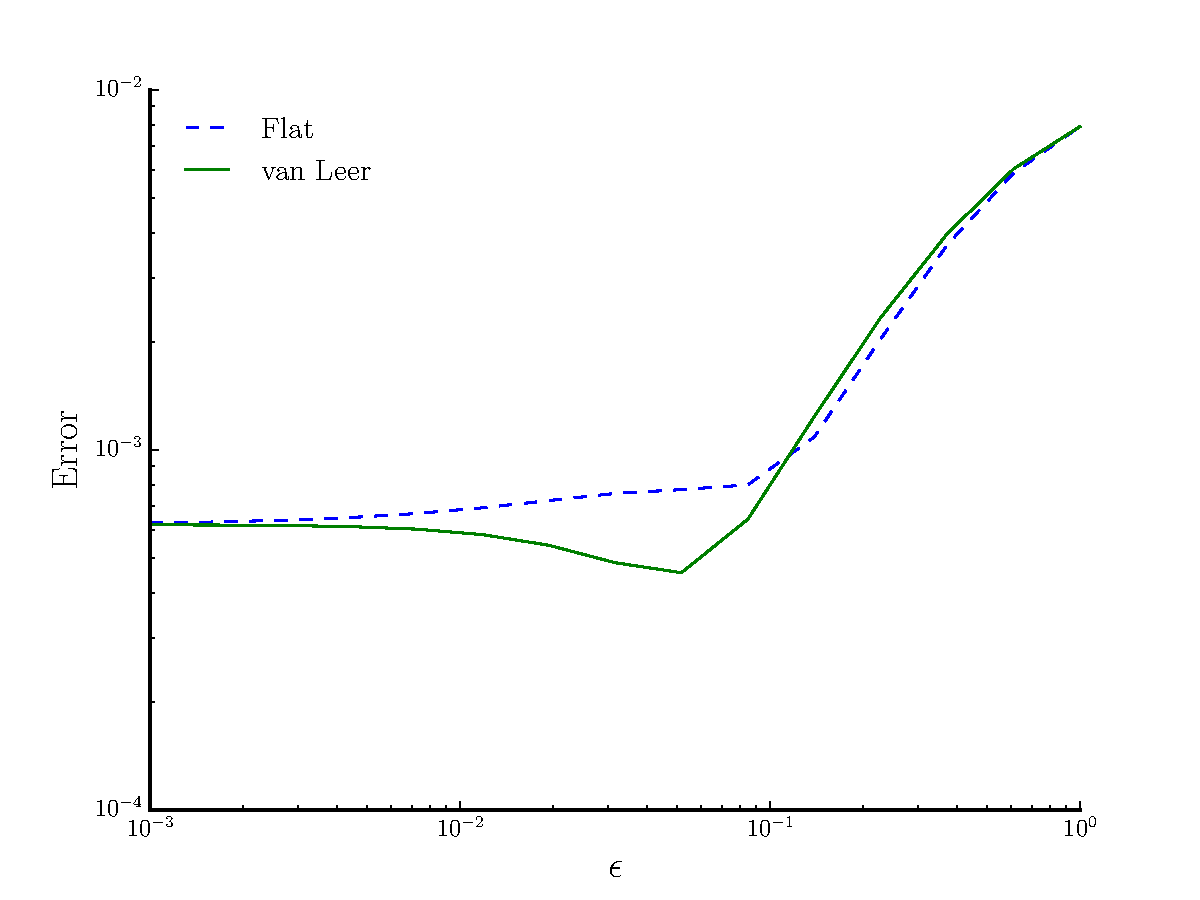
\includegraphics[width=.75\textwidth]{figs/dl_err.pdf}
		\caption{The error between the VEF methods and the exact diffusion solution as $\epsilon \rightarrow 0$. }
		\label{fig:dl_err}
	\end{figure}